Da das Projekt mehrere Ebenen(Elektronisch, mechanisch und Signaltechnisch) umfasst, wurde versucht, alle Möglichkeiten zu jedem Sub-Element in einem morphologischen Kasten aufzuzeichnen. Dieser ist in Abbildung \ref{pic:morphologischer_kasten} zu sehen. Aus diesen konnten nun verschiedene Varianten generiert und bewertet werden.
\begin{figure}[H]
	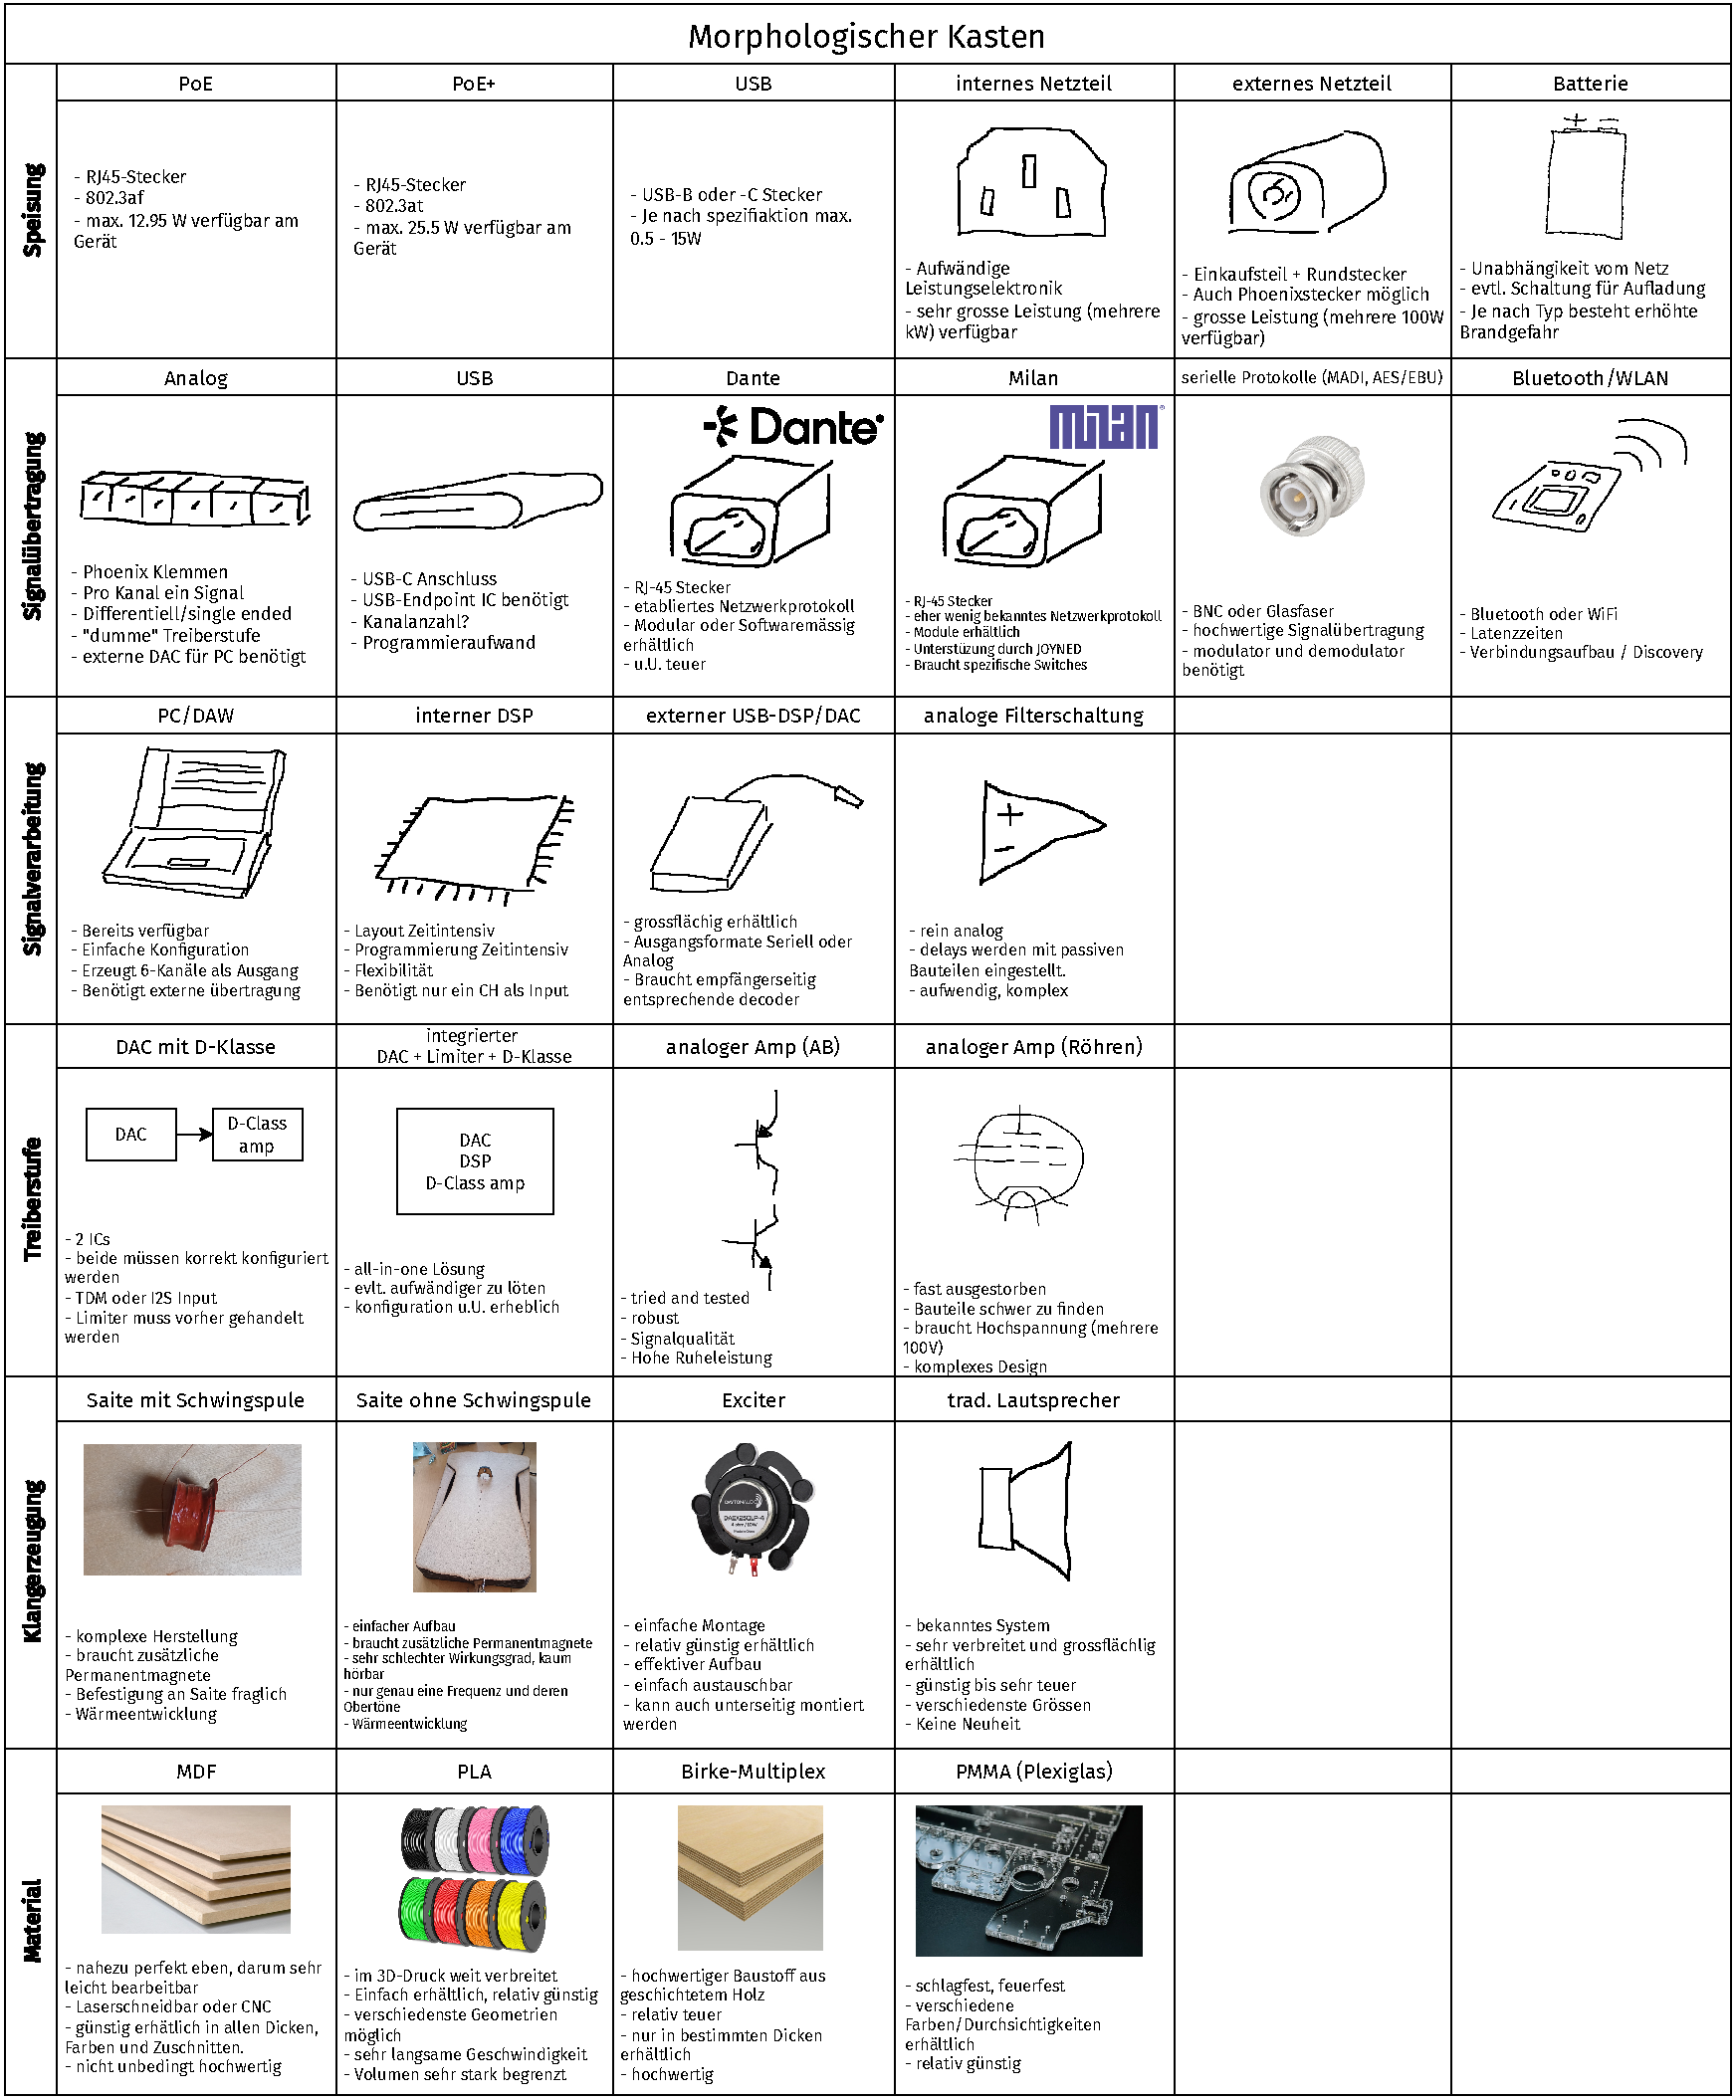
\includegraphics[width=\textwidth]{pictures/morphologischer_kasten.pdf}
	\caption{Der morphologische Kasten}
	\label{pic:morphologischer_kasten}
\end{figure}